\subsubsection{Greater Than Sudoku}

I've found this on \url{http://www.killersudokuonline.com}:

\begin{figure}[H]
\centering
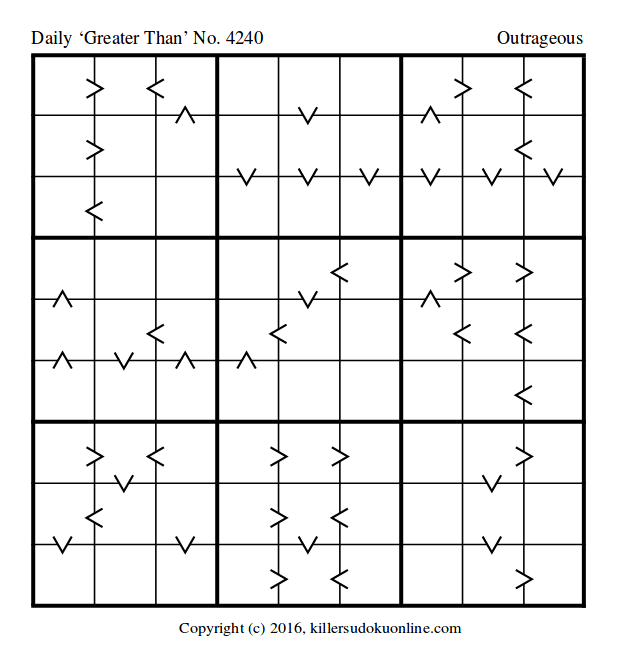
\includegraphics[scale=0.6]{puzzles/sudoku/GT/puzzle.png}
\caption{}
\end{figure}

% TODO \ref
It can be solved easily with Z3. I've took the same piece of code I used for the usual Sudoku: ().
% ( _HTML_LINK_AS_IS(`https://github.com/DennisYurichev/SAT_SMT_article/blob/master/SMT/sudoku2.py'), 

... and added this:

\begin{lstlisting}
...

"""
Subsquares:

------------------------------
         |          |         
 1,1     | 1,2      | 1,3     
         |          |         
------------------------------
         |          |         
 2,1     | 2,2      | 2,3     
         |          |         
------------------------------
         |          |         
 3,1     | 3,2      | 3,3     
         |          |         
------------------------------
"""

# from http://www.killersudokuonline.com/puzzles/2017/puzzle-GD4hzi164344.pdf

# subsquare 1,1:
s.add(cells[0][0]>cells[0][1])
s.add(cells[1][0]>cells[1][1])
s.add(cells[2][0]<cells[2][1])

s.add(cells[0][1]<cells[0][2])
s.add(cells[0][2]<cells[1][2])

# subsquare 1,2:
s.add(cells[0][4]>cells[1][4])
s.add(cells[1][3]>cells[2][3])
s.add(cells[1][4]>cells[2][4])
s.add(cells[1][5]>cells[2][5])

# subsquare 1,3:
s.add(cells[0][6]>cells[0][7])
s.add(cells[0][7]<cells[0][8])
s.add(cells[0][6]<cells[1][6])
s.add(cells[1][7]<cells[1][8])
s.add(cells[1][6]>cells[2][6])
s.add(cells[1][7]>cells[2][7])
s.add(cells[1][8]>cells[2][8])

# subsquare 2,1:
s.add(cells[3][0]<cells[4][0])
s.add(cells[4][0]<cells[5][0])
s.add(cells[4][1]<cells[4][2])
s.add(cells[4][0]<cells[5][0])
s.add(cells[4][1]>cells[5][1])
s.add(cells[4][2]<cells[5][2])

# subsquare 2,2:
s.add(cells[3][4]>cells[4][4])
s.add(cells[3][4]<cells[3][5])
s.add(cells[4][3]<cells[4][4])
s.add(cells[4][3]<cells[5][3])

# subsquare 2,3:
s.add(cells[3][6]>cells[3][7])
s.add(cells[3][7]>cells[3][8])
s.add(cells[3][6]>cells[4][6])
s.add(cells[4][6]<cells[4][7])
s.add(cells[4][7]<cells[4][8])
s.add(cells[5][7]<cells[5][8])

# subsquare 3,1:
s.add(cells[6][0]>cells[6][1])
s.add(cells[6][1]<cells[6][2])
s.add(cells[6][1]>cells[7][1])
s.add(cells[7][0]<cells[7][1])
s.add(cells[7][0]>cells[8][0])
s.add(cells[7][2]>cells[8][2])

# subsquare 3,2:
s.add(cells[6][3]>cells[6][4])
s.add(cells[6][4]>cells[6][5])
s.add(cells[7][3]>cells[7][4])
s.add(cells[7][4]<cells[7][5])
s.add(cells[8][3]>cells[8][4])
s.add(cells[8][4]<cells[8][5])
s.add(cells[7][4]>cells[8][4])

# subsquare 3,3:
s.add(cells[6][7]>cells[6][8])
s.add(cells[6][7]>cells[7][7])
s.add(cells[7][7]>cells[8][7])
s.add(cells[8][7]>cells[8][8])

...
\end{lstlisting}

( The full file: \url{https://github.com/DennisYurichev/SAT_SMT_by_example/blob/master/puzzles/sudoku/GT/sudoku_GT.py} )

The puzzle marked as ``Outrageous'' (for humans?), however it took $\approx 30$ seconds
on my old Intel Xeon E3-1220 3.10GHz to solve it:

\begin{lstlisting}
7 3 4 6 9 2 5 1 8
2 1 5 8 3 7 9 4 6
6 8 9 5 1 4 7 2 3
1 7 3 2 8 9 6 5 4
5 4 6 1 7 3 2 8 9
9 2 8 4 5 6 1 3 7
8 6 7 3 2 1 4 9 5
4 5 2 9 6 8 3 7 1
3 9 1 7 4 5 8 6 2
\end{lstlisting}

